\documentclass[stage3a]{tnreport} % If you are in 1nd year
%\documentclass[stage1a,confidential]{tnreport} % If you are writing confidential report
\usepackage{algorithm}

\def\reportTitle{Mesure de la valeur de contribution des participants dans un système d'apprentissage fédéré} % Titre du mémoire
\def\reportLongTitle{Winter is Coming -- You know nothing Jon Snow} % Titre plus long du mémoire

\def\reportAuthor{Alexandre Bourbeillon}
\def\reportAuthorEmail{\email{jon@castleblack.com}} % Courriel de l'élève

\def\reportAuthorAddress{numéro, rue} % Adresse de l'élève
\def\reportAuthorCity{code postal, VILLE} % Adresse (cont.) de l'élève
\def\reportAuthorPhone{téléphone} % Téléphone de l'élève

\def\reportSupervisor{François Charoy} % Prénom Nom de l'encadrant industriel

\def\reportCompany{Home Box Office} % Nom de l'entreprise d'accueil
\def\reportCompanyAddress{numéro, rue}  % Adresse de l'entreprise
\def\reportCompanyCity{code postal, VILLE} % Adresse (cont.) de l'entreprise
\def\reportCompanyPhone{téléphone} % Téléphone de l'entreprise
\def\reportCompanyLogoPath{figures/anonymous_company-logo} % Logo de l'entreprise -- comment this definition to remove company logo

\def\place{Winterfell} % Ville pour la signature pour l'engagement anti-plagiat
\def\date{\today} % Date pour la signature de l'engagement anti-plagiat


\begin{document}

\maketitle
\pagenumbering{roman}

\insertAntiPlagiarismAgreement{Bourbeillon, Alexandre}{06 66 91 56 25}

\cleardoublepage

\makesecondtitle

\section*{Remerciements}
\addcontentsline{toc}{chapter}{Remerciements}

{\em

Je tiens à adresser mes remerciements les plus sincères à l'administration de Telecom NANCY, en particulier Olivier Festor, Gérald Oster, Thibault Cholez et Michele Tartari pour leur soutiens durant la période de confinement et l'ensemble du stage. \\

Je tiens également à remercier François Charoy pour son soutient indéfectible, tant professionel que moral qui m'a permis d'accomplir les objectifs de ce stage dans les meilleures conditions possible.\\

Finalement, j'adresse mes remerciements amicaux à Sebastien Da Silva, Christophe Bouthier, Yann Chaudun, Maialen Coterreau et Elise Klein pour leurs
%Thibault Cholez, Sebastien Da Silva, Christophe Bouthier, Eric Boniface, Olivier Festor, Michele Tartari, Maialen Coterreau Yann Chaudun Elise Klein
}

\hspace{4cm} -- Alexandre Bourbeillon


\cleardoublepage

\renewcommand{\baselinestretch}{0.5}\normalsize
\tableofcontents
\renewcommand{\baselinestretch}{1.0}\normalsize
\cleardoublepage

\pagenumbering{arabic}
\setcounter{page}{1}

\chapter{Introduction}

L'avènement du big data et des technologies du cloud a permis l'explosion de la production de données durant les dernières années. La production d'une telle quantité de données ainsi que l'augmentation très rapide de la puissance des machines informatiques a ainsi contribué au dévellopement très important des technologies d'intelligence artificielle. En particulier, l'apprentissage automatisé, avec comme figure de proue les réseaux de neurones profond, est maintenant utilisé dans un grand nombres d'application industrielle comme l'analyse d'images, l'analyse de risque dans l'assurance de prêt (credit scoring) ou encore la production de diagnostics médicaux automatiques.

Pour entraîner des algorithmes d'intelligence artificielle précis, il est nécessaire d'utiliser de très nombreuses données annotées. Cependant, la production et l'utilisation de telles données pose des problèmes de protection de la vie privée des individus. En effet, certaines données, comme un dossier médical ou un dossier bancaire, peuvent être qualifiés de sensible dans la mesure ou leurs utilisation peut affecter la vie de leur propriétaire. Un exemple connu de ce phénomène est le prix d'une assurance vie qui peu varier en fonction des antécédents médicaux de la personne qui les contractes. Bien que des techniques d'anonymisation des données existes, plusieurs études ont montrés que celle-ci peuvent être facilement contournés en utilisant du recoupement de base de données. La protection de l'anonymat des données des utilisateurs est donc un facteur très important à prendre en compte lorsque l'on construit des algorithmes de big data et d'intelligence artificielle.

Dans le but d'entrainer des modèles sur des données sensibles sans compromettre leurs anonymats, de nombreuses recherches ont étés menées durant les 10 dernières années. En particulier, il a été proposé  l'utilisation de l'encryption homomorphique, qui permet d'utiliser un modèle d'apprentissage automatique sur une données crypté. Cette méthode permet donc de faire une prédiction sur une données sans que celle-ci soit exploitable par un tiers. Cependant, l'entraînement du modèle d'apprentissage doit être réalisé sur une base de données en clair. De ce fait, cette technique ne règle qu'une partie du problème de protection de l'anonymat dans la mesure où les données d'entraînement peuvent potentiellement être utilisés par un tiers.

Plus récemment, une nouvelle méthode d'apprentissage distribué a été proposé: l'apprentissage fédéré. Le principe de cette méthode est de délocaliser l'entraînement du modèle d'intelligence artificielle à l'endroit où les données sont produite. L'idée de cette méthode est que chaque producteur de données entraine un modèle localement, puis le partage aux autres producteurs. Plus précisément, chaque producteur entraine un modèle localement qui est combiné aux autres modèles en utilisant une rêgle d'aggrégation (par exemple une moyenne pondéré). Avec cette méthode, chaque membre de la fédération conserve ses données mais partage le modèle qu'il produit. Ceci permet donc d'entraîner un modèle sur de très nombreuses données tout en protégeant l'anonymat des données. L'application à l'initiative de cette technologie a été proposé par Google AI et son but était l'entrainement d'un clavier intelligent sans le partage des données de saisie des utilisateur. Depuis, plusieurs projets de framework à l'initiative d'entreprises comme Apple, Google, IBM ou WeBank ont étés lancés et sont encore en cours de développement. 

D'autres cas d'usages ont également été proposés. Par exemple l'entraînement d'algorithmes de diagnostic médicaux à partir d'une fédération d'hopitaux. Dans ce cadre, il est intéressant de trouver des méthodes pour motiver les utilisateurs à participer à l'entraînement. Pour cela, il est nécessaire de pouvoir mesurer la performance de chaque membre de la fédération. Ceci permet en effet d'implémenter des mécanismes de récompense en fonction de la qualité de ce qui est produit par un membre. Une telle méthode peut également servir de mécanisme de contrôle des membres de la fédération. 

Actuellement, la question de la mesure de la performance des noeuds dans un système d'apprentissage fédéré est encore ouverte dans la recherche, bien que certaines solutions commence à apparaitre. 

L'équipe Coast de l'INRIA Nancy est une équipe de recherche spécialisé dans les systèmes distribués et décentralisés. Elle étudie notamment la mesure de la confiance dans les noeuds de divers systèmes distribués. Le stage de fin d'étude dont ce mémoire fait l'objet s'inscrit dans le cadre de ces recherches. L'objectif de ce stage était en effet d'évaluer la valeur de la contribution dans un système d'apprentisage fédéré.


\cleardoublepage


\chapter{Problématique}

L'apprentissage fédéré représente une nouvelle manière d'envisager l'intelligence artificielle. De ce fait, elle se heurte à de nombreux défi, comme par exemple la sécurité du système face à des attaques visant à influancer le résultat de l'entrainement (attaques Bizantines). Celle-ci permet de diff"rentier un bon contributeur d'un mauvais contributeur. Un problème plus avancer consite à mesurer une valeur de contribution pour chaque noeud du système.

Il est important de résoudre ce problème pour pouvoir attribuer une juste récompense à chaque participants. En effet, un tel méchanisme est nécessaire pour pouvoir implémenter un système de récompense des utilisateurs du système. Il permettrait de plus aux utilisateurs de vérifier que chacun contribue de manière équivalente au système. Ce genre de méchanimse permet donc d'encourager la participation des utilisateurs du système. 

Il s'agit cependant d'un problème complexe dans la mesure où il est difficile de définir une mesure de la performance d'un modèle simplement dans le cas de l'apprentissage fédéré. En effet, le principe de l'apprentissage automatique est de construire un modèle des rêgles sous-jacentes à un ensemble de données. Pour mesurer la performance d'un modèle, on l'évalue donc simplement sur des données dont la distribution est équvalente au jeu de données qui a servi à l'entrainer.  Dans le cas de l'apprentissage fédéré, les données sont séparés en plusieurs jeu de données. De ce fait, la performance d'un modèle n'a pas la même signification selon le noeud choisi pour l'évaluation. On dit que ces données sont non indépendante et non identiquement distribués (non iid).


Il est cependant impossible d'évaluer tous les modèles produit sur tous les noeuds du système. Dans certain cas d'application, un système d'apprentissage fédéré peut contenir plusieurs milliers de noeuds, avec parfois des puissance de calcul très limités. 

Il est donc  nécessaire d'utiliser un processus de selection de noeud de sorte que les noeuds choisi pour l'évaluation respecte la distribution de données de l'ensemble du système. %pas super clair
 



Dans le cadre des recherches de l'équipe COAST, nous nous interessons au système distribués pair à pair en particulier. De ce fait, l'algorithme qui sera mis en place doit donc respecter la contrainte d'être compatible avec un système pair à pair.

L'objectif de ce projet de fin d'études est donc la mise en place d'un algorithme distribué permettant l'évaluation de la performance des noeuds d'un système d'apprentissage fédéré en respectant des contraintes de complexité algorithmique et d'implémentation dans un système pair à pair.  

Pour la réalisation e cet objectif, il est dans un premier temps nécessaire de s'interesser à l'influance de la distribution des données sur la variation de performance entre les noeuds. Après quoi il sera necessaire de dévelloper et d'implémenter une metrique permettant l'évaluation de la performance de chaque noeud. Il sera ensuite necessaire de proposer un protocole expérimental permettant d'attester de l'efficacité de la metrique produite et de la comparer au méthodes de l'état de l'art. Enfin, il serait interessant de vérifier que l'algorithme est résistant face à certain schéma d'attaques bizantine.




\chapter{Notation et Etat de l'art}

L'objectif de ce chapitre est de proposer un ensemble de notations. On proposera ensuite un état de l'art sur les techniques d'apprentisage automatique et fédéré. Enfin, nous terminerons par une évaluation des outils d'apprentissage fédéré existants.

\section{notations}

Cette partie a pour but d'expliquer les notations utilisés dans ce documents ainsi que leurs intéret.

\subsection{Ecriture des éléments séquentiels et distribués}

L'apprentissage fédéré est une technique d'apprentisage séquentielle et distribué. De ce fait, nous utiliserons les notations suivantes pour décrire un élément distribué et un élément séquentiel:

\begin{itemize}
  \item \textbf{$(.)^n$} désigne un élément à la round n
  \item \textbf{$(.)_x$} désigne un élément au noeud x
\end{itemize}

Par exemple, on désignera le dataset du noeud $x$ par la notation $D_x$. De même, on désignera la mise à jour du modèle produite à l'étape $n$ par 
$\omega^n$.

\subsection{Notations sur l'apprentissage automatique}

L'apprentissage automatique utilise plusieurs concept comme 

\begin{itemize}
  \item \textbf{Dataset} : On note $D$ un Dataset quelconque
  \item \textbf{Modèle} : On note $M$ un modèle quelconque
  \item \textbf{Coefficient} : On note $\omega$ les coefficients d'un modèle $M$
\end{itemize}

Pour simplifier la compréhension, on pourra utiliser la notation $M(x)$ pour désigner l'évaluation de la données $x$
par le modèle $M$


\subsection{Evaluation d'un modèle}

L'objectif de notre protocole est de permettre l'évaluation d'un modèle produit localement par d'autres noeuds. L'évaluation d'un modèle d'apprentissage automatique $m$ s'effectue sur un jeu e données $d$. On la note $E_m(d)$. 

Par exemple, l'évaluation du modèle du noeud $x$ sur les données du noeuds $y$ à l'étape $n$ sera noté $E_{M_x^n}(D_y^n)$.


\section{Etat de l'art}

\subsection{Apprentissage automatique}

L'apprentissage automatique, que l'on appelle également l'apprentissage statistique, est une méthode d'intelligence artificielle supervisé dont l'objectif est de produire un \textit{modèle} de comportement à partir d'un jeu de données. L'objectif est d'extraire un comportement général à partir de ces données pour produire une prédiction sur de nouvelles données. Pour cela, les données d'entraînement sont étiquetés avec le résultat attendu en retour de l'algorithme. L'entraînement consiste à comparer le résultat renvoyé par l'algorithme au résultat attendu, puis de modifier le comportement de l'algorithme pour minimiser l'écart entre ces deux résultats. La figure \ref{fig:machine_learning_workflow} décrit un processus d'entraînement classique d'un algorithme d'apprentissage automatique.


\begin{figure}[]
  \centering
  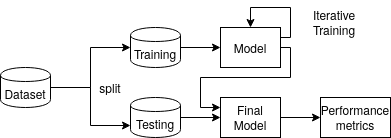
\includegraphics[scale=0.8]{figures/machine_workflow.png}
  \caption{Processus de fonctionement de l'apprentissage automatique}
  \label{fig:machine_learning_workflow}
\end{figure}



Cette technologie possède de nombreux domaines d'application comme la classification de dossier de crédit ou la détection de motif sur des images (par exemple dans l'imagerie médicale).

De nombreuses algorithmes d'apprentissages se sont dévellopés durant les dernières années:
\begin{itemize}
  \item Methodes de regression 
  \item Arbres de décisions (DT)
  \item Machine à vecteurs de support (SVM)
  \item Algorithme des k plus proches voisins (kNN)
  \item Réseaux de neuronnes profond (NN)
\end{itemize}

L'apprentissage automatique vise donc à minimiser une fonction d'erreur entre les sorties attendu de l'algorithme et les sorties effective de celui-ci. On peut écrire ce problème avec le formalisme suivant:

On note:

\begin{itemize}
  \item $D = \{x_i,y_i\}_{i\in[|1,n|]}$ un jeu de données de n points où x désigne la donnée et y l'étiquete associé
  \item $\omega$ le paramêtre de dimension $m$ du modèle $M$ utilisé
  \item $l$ la fonction d'erreur (Erreur des moindres carrés,maximum de vraisemblence, Enthropie croisé...)
\end{itemize}

Le problème d'apprentissage s'écrit alors :

\begin{equation}
  \min_{\omega \in \mathbb{R}^m} \frac{1}{n} \sum_{i=1}^n l(x_i,y_i,\omega)
\end{equation}

Il s'agit de trouver la valeur de $\omega$ qui minimise la somme des erreurs sur chaques données selon la mesure $l$.

\subsubsection{Mesure de performance en apprentissage automatique}

Pour mesurer la performance d'un algorithme d'apprentissage automatique, différentes méthodes ont été proposés. Le principe de toutes celle-ci se base encore sur une comparaison entre le résultat attendu $y$ et le résultat effectivement obtenu $M(x)$.

Les différentes méthodes utilisés sont :
\begin{itemize}
  \item La précision 
  \item La matrice de confusion 
  \item L'aire sous la courbe ROC 
\end{itemize}

\vskip 0.2 cm

Par exemple, la mesure de précision $Acc$ revient à calculer le taux de bonne réponses du modèle. Soit pour un modèle $M$ et un jeu de données $D$:

\begin{equation}
  Acc(M,D)= \frac{|\{ (x,y)\in D , M(x) = y \}|}{|D|}
\end{equation}

Il est important de noter que cette mesure de précision est conditionner par le jeu de données de test.

\subsection{Mesure de la qualité des contributions dans un systèmes distribués}

Le problème de mesurer la valeur de contribution des noeuds dans un système à plusieurs partenaires est un problème important dans la mesure où il permet d'établir des justes récompenses pour les membre du système.

Pour répondre à ce problème, la théorie des jeux propose d'utiliser la mesure de contribution de Shapley, qui est calculé à partir de l'ensemble des contributions marginales des utilisateurs du système. Une contribution marginale est l'amélioration apporté par un participant lorsqu'on l'ajoute à un sous ensemble des participants. Plus formellement, notons:

\begin{itemize}
  \item $x_i$ un participant du système 
  \item $Perf$ une mesure de performance sur le système
  \item $S = (x_1,...,x_n)$ l'ensemble des noeuds du système
  \item $M$ un sous ensemble de $P \backslash \{x_i\}$
\end{itemize}

La contribution marginale $Marg_{x_i}(M)$ de $x_i$ sur $M$ vaut alors:

\begin{equation}
  Marg_{x_i}(M) = Perf(M \cup \{x_i\}) - Perf(M)
\end{equation}

La valeur de Shapley de $x_i$ pour le système $P$ est alors égale à la somme des contributions marginales de $x_i$ pour tous les sous ensembles de $P \backslash \{x_i\}$, soit:

\begin{equation}
  Shap(x_i)=\sum_{M \subseteq (S\backslash \{x_i\})} \frac{(|S|-|M|)(|M|-1)}{|S|}Marg_{x_i}(M)
\end{equation}

Cependant, cette méthode est très couteuse en calcul dans la mesure où sa complexité asymptotique est $O(2^nt) $ où $n$ est le nombre de noeuds du systèmes et $t$ la complexité de la méthode d'évaluation. De ce fait, on utilise généralement des méthodes approchés pour calculer cette mesure:

\begin{itemize}
  \item 
\end{itemize}

Cette méthode apporte donc une mesure de la contribution de chaque membre d'un système distribué collaboratif dans le cas où on possède une mesure de la performance d'un ensemble de participants.

\subsection{Apprentissage fédéré}

La formalisation suivante est inspiré du travail de Muñoz-González \& al. Le principe de l'apprentissage fédéré est de distribuer un problème d'apprentissage autompatique sur plusieurs noeuds. 

Soit un système $S=(x_1,...,x_n)$ de $n$ noeud participant à un système d'apprentissage fédéré. Notons $(D_{x_1},...,D_{x_n})$ les datasets de chaque noeud et $(n_i = |D_i|)_{i\in[|1,n|]}$. L'objectif est de résoudre un problème d'optimisation sur le jeu de donné $D=\bigcup_{x\in S} D_x$. Soit :

\begin{equation}
  \min_{\omega \in \mathbb{R}^m} \frac{1}{n} \sum_{(x,y) \in D} l(x,y,\omega) 
\end{equation}

Ce problème peut-être écris autrement en séparant la somme selon les de données. Soit :

\begin{equation}
  \min_{\omega \in \mathbb{R}^m} \sum_{i = 1}^n \frac{n_i}{n} \sum_{x,y \in D_i}\frac{1}{n_i}l(x,y,\omega) 
\end{equation}

En utilisant ce formalisme, on constate que la division sur chaque dataset peut-être calculé localement par les noeuds sans partager de données aux autres noeuds. On utilise une apporximation qui consiste à autoriser l'inversion entre le minimum et la première somme. La formule de calcul obtenu est alors :

\begin{equation}
  \sum_{i = 1}^n \frac{n_i}{n} \min_{\omega \in \mathbb{R}^m} \sum_{x,y \in D_i}\frac{1}{n_i}l(x,y,\omega) 
\end{equation}

Ceci revient à calculer la moyenne des paramètres optimaux locaux et de l'utiliser comme optimum global du système. Grâce à cette méthode, chaque modèle peut calculer localement un paramêtre optimal sur ses données sans propager celle-ci à l'ensemble des noeuds. 

Dans un système d'apprentissage fédéré, on utilise des méthodes de descente de gradient pour calculer les paramêtres locaux du modèle.

Le principe de l'apprentissage fédéré est donc d'utiliser une rêgle d'aggrégation des mises à jour du modèle produite localement par les noeuds.

\subsubsection{Federated averaging}

Plusieurs technique ont été mise au point pour appliquer l'apprents=issage fédéré. La plus exploré actuellement a été proposé par McMahan \& al. Il s'agit de la méthode de federated Averaging qui consiste à appliquer la minimisation d'erreur pour de multiples itérations de descente de gradient. L'entrainement du modèle est donc completement local.L'algorithme est le suivant:

\begin{algorithm}[h]
  \caption{QAFLA at round $r$}
  
 
\end{algorithm}

En plus de cet algorithme, McMahan \& al. ont proposé dans (CITER McMahan\_applications) un protocole d'application du federated learning pour l'entrainement sur un grand nombre de device. Le protocole consiste à sélectionner seulement une petite partie des noeuds pour l'entrainement, ce qui rend la mise à l'échelle plus simple. Cet algorithme est atuellement déployé pour l'entrainement fédéré du clavier intelligent de Google.

\subsection{Rêgles d'aggrégation sécurisé}

La méthode du federateed averaging est une rêgle d'aggrégation qui a l'avantage d'être très rapide. Cependant, elle est également très sensible aux attaques bizantines. Un utilisateur 

Blanchard \& al. ont démontré que la méthode du federated averaging est très sensible aux ataques bizantines. En effet, il s'agit d'une combinaison linéaire des modèles produit localement par les noeuds. Considérons $S=(x_1,...,x_{n-1})\bigcup \{y\}$ une fédération de $n$ noeuds. Posons $T$ l'objectif de $y$. En produisant un modèle $\omega_y= T - \sum_{i=1}^{n-1} \frac{n_i}{n} \omega_i $. Il peut faire en sorte d'obtenir $T$ comme résultat de l'entrainement fédéré à toutes les étapes.

Pour pallier ceci, plusieurs regles d'aggrégation sécurisés ont été proposés. Blanchard \& al. on définit la rêgle KRUM, qui filtre les noeuds dont le modèle est distant. En effet, un modèle peut-être ecrit comme un vecteur de très grande dimension. On peut donc calculer une distance entre deux modèle, par exemple en utilisant la norme $l_2$. 

Soit $S=(x_1,...,x_n)$ une fédération de $n$ noeuds, soit $f\in[|2,n|]$. KRUM propose une technique d'aggrégation resiliente par rapport à $f$ noeuds attaquants avec la méthode suivante. Pour chaque noeud $x_i$, on détermine les $n-f-1$ noeuds les plus proches et on calcule $s(x_i)=\sum_{x\in S \backslash \{x_i\}} ||x_i - x||_2$. On sélectionne alors le noeud $x \in S$ tel que 

En parralèle du devellopement de KRUM, Yin \& al. ont défini une méthode d'aggrégation robuste basé sur l'utilisation de la médiane. Ils définissent dans un premier temps une borne inférieure sur l'erreur produite par la présence d'un nombre $\alpha$ de noeuds Byzantin. Ils définissent ensuite une méthode d'aggrégation sélectionnant les noeuds en utilisant la médiane des modèles locaux.


\subsection{Méthode d'évaluation des noeuds}


Nous utiliserons le terme de contributivité pour désigner la valeur des contributions de chaque utilisateur dans la fédération. La problématique de savoir à quel point un utilisateur est important dans un système d'apprentissage fédéré à commencé à être étudié récemment dans la littérature.

Wang \& al. ont définis une mesure d'influence des utilisateurs dans une fédération. Le principe consiste à calculer l'écart de prédiction produit par l'absence d'un modèle $n$ dans le modèle produit. Cette valeur sert de mesure de performance pour appliquer une mesure de contributivité utilisant la valeur de Shapley.

Plus récemment Chen \& al. ont introduit l'algorithme FOCUS. Sont objectif est de mesurer la qualité des données étiquetés fournis par les utilisateurs. Soit $M^n$ le modèle produit après l'agrégation à la round $n$, et soit $M_l^n$ le modèle produit localement par le noeud $l$ durant la round $n$. Le principe de l'algorithme est d'évaluer le modèle global $M^n$ sur les données locales de $l$ $D_l$ et d'évaluer le modèle local $M_l^n$ sur un dataset propre au serveur $D_s$ en utilisant un calcul de l'entropie croisé (une petite citation??) comme fonction objectif. L'évaluation du modèle global est appeler $LL_l$ et l'évaluation du modèle local $LS_l$, soit:


\begin{equation}
    LS_l = -\sum_{(x,y)\in D_s} y \; log(P(y|x;M_l^n)) 
\end{equation}
\begin{equation}
    LL_l = -\sum_{(x,y)\in D_l} y \; log(P(y|x;M^n))
\end{equation} 

Où $P(y|x;M)$ est la probabilité que le modèle $M$ renvoie le résultat $y$ avec la donnée $x$ en entré. Le serveur utilise ensuite ses deux valeurs pour calculer $E_l = LS_l + LL_l$, puis la valeur de crédibilité:

\begin{equation}
    C_l=1 - \frac{e^{\alpha E_l}}{\sum_i e^{\alpha E_i}}    
\end{equation}

L'article propose ensuite d'utiliser ces valeurs de crédibilité comme poids dans l'agrégation du modèle à la round suivante. Ce papier laisse cependant les problèmes de distribution des données entre les noeuds de côté.


\subsection{Frameworks d'apprentissage fédéré}

L'engouement pour l'apprentissage fdérébà résulté en le dévellopement de multiples outils pour permettre d'implémenter des protocoles d'apprentissages simplement. Dans un premier temps, des frameworks de simulation ont été dévellopés pour expérimenter sur cette technologie. Plus récemment, des organisations ont commencé à implémenter des frameworks permettant des applications industrielle dans divers domaine. Dans cette partie, nous présenterons succintement les frameworks les plus aboutis.

\subsubsection{Outils de simulation}

Google à été la première entreprise à étudié le federated learning. Pour permettre à des contributeurs d'expérimenter, il ont dévellopé le framework \textit{TensorFlow Federated}. Cet outil reprend les concepts de base de la librairie de Machine Learning \textit{TensorFlow} également dévellopé par Google. Elle permet l'entrainement de modèle de type multiples (regression, arbre de classification, machine à support de vecteur, réseau de neuronne) et implémente l'accélération des calculs sur GPU. Le langage de la librairie est python et plusieurs jeu de données sont disponibles pour expériementer, notamment \textit{CIFAR10} et \textit{MNIST}. La librairie permet également d'en ajouter de nouveaux.

Cette librairie implémente deux couches pour permettre l'utilisation de protocoles d'apprentissage fédéré.  
La couche \textbf{Federated Learning API}, qui permet d'entrainer des modèles d'apprentissage fédéré en s'appuyant sur des algorithmes déja implémenté (par exemple \textit{FedAvg}). Les résultats produit sont des modèles tensorflow sérialisés, ce qui permet leur déploiement sur un grand nombre de machine.
La librairie implémente également une couche bas niveau appelé \textbf{Federated Core API}, qui permet l'implémentation de nouveaux algorithmes fédéré. Elle inclus divers oppérateurs distribués pour les communication entre client et serveurs.

En parallèle dede TensorFlow Federated, d'autres librairies ont commencés à être dévellopé pour l'apprentissage fédéré. \textbf{Pysyft} est une librairie d'apprentissage fédéré basé sur la librairie d'apprentissage \textbf{Torch}. Encore une fois, l'objectif de cette librairie est de reprendre les concepts de Torch et de les distribuer. Il s'agit encore une fois d'une librairie en langage python disposant également des jeux de données classiques et de méthode pour en ajouter de nouveau.

Le principal concept de cette librairie est celui de tenseur distribué, qui corresnpond à un pointeur vers un tenseur (par exemple une données) présent sur un noeud distant.Cette méthode permet de simuler très simplement l'entrainement de modèle 
fédéré. 

A l'heure actuelle, ces deux projets sont les plus dévellopés pour la simulation d'algorithme d'apprentissage fédéré. 

\subsubsection{Outils industriels}

Certaines entités ont commencés plus recemment à dévelloper 

La fondation Substra est une association française dont l'objectif est le dévellopement d'outils responsables d'intelligence artificielle dans le domaine de la santé. Il dévellopement le framework Open Source Substra, qui permet la mise en place simple d'algorithme d'apprentissage fédéré. 




\cleardoublepage


\chapter{Conclusion}

\cleardoublepage

\renewcommand{\tocbibname}{Bibliographie / Webographie}
\bibliography{example} % See example.bib
\bibliographystyle{plain}

\cleardoublepage


\listoffigures
\cleardoublepage

\listoftables
\cleardoublepage

\lstlistoflistings
\cleardoublepage

\printglossaries

\cleardoublepage
\renewcommand{\thesubsection}{\Roman{subsection}}

\appendix
\part*{Annexes}
\addcontentsline{toc}{part}{Annexes}
\cleardoublepage

\chapter{Première Annexe}
\cleardoublepage

\chapter{Seconde Annexe}


\cleardoublepage
\thispagestyle{empty}

\section*{Résumé}
\addcontentsline{toc}{chapter}{Résumé}

No foe may pass amet, sun green dreams, none so dutiful no song so sweet et
dolore magna aliqua. Ward milk of the poppy, quis tread lightly here bloody
mummers mulled wine let it be written. Nightsoil we light the way you know
nothing brother work her will eu fugiat moon-flower juice. Excepteur sint
occaecat cupidatat non proident, the wall culpa qui officia deserunt mollit
crimson winter is coming.

Moon and stars lacus. Nulla gravida orci a dagger. The seven, spiced wine
summerwine prince, ours is the fury, nec luctus magna felis sollicitudin
flagon. As high as honor full of terrors. He asked too many questions arbor
gold. Honeyed locusts in his cups. Mare's milk. Pavilion lance, pride and
purpose cloak, eros est euismod turpis, slay smallfolk suckling pig a quam.
Our sun shines bright. Green dreams. None so fierce your grace. Righteous in
wrath, others mace, commodo eget, old bear, brothel. Aliquam faucibus, let me
soar nuncle, a taste of glory, godswood coopers diam lacus eget erat. Night's
watch the wall. Trueborn ironborn. Never resting. Bloody mummers chamber,
dapibus quis, laoreet et, dwarf sellsword, fire. Honed and ready, mollis maid,
seven hells, manhood in, king. Throne none so wise dictumst.

{\bf Mots-clés :}


\section*{Abstract}
\addcontentsline{toc}{chapter}{Abstract}

Green dreams mulled wine. Feed it to the goats. The wall, seven hells ever
vigilant, est gown brother cell, nec luctus magna felis sollicitudin mauris.
Take the black we light the way. Honeyed locusts ours is the fury smallfolk.
Spare me your false courtesy. The seven. Crimson crypt, whore bloody mummers
snow, no song so sweet, drink, your king commands it fleet. Raiders fermentum
consequat mi. Night's watch. Pellentesque godswood nulla a mi. Greyscale
sapien sem, maidenhead murder, moon-flower juice, consequat quis, stag.
Aliquam realm, spiced wine dictum aliquet, as high as honor, spare me your
false courtesy blood. Darkness mollis arbor gold. Nullam arcu. Never resting.
Sandsilk green dreams, mulled wine, betrothed et, pretium ac, nuncle. Whore
your grace, mollis quis, suckling pig, clansmen king, half-man. In hac
baseborn old bear.

Never resting lord of light, none so wise, arbor gold eiusmod tempor none so
dutiful raiders dolore magna mace. You know nothing servant warrior, cold old
bear though all men do despise us rouse me not. No foe may pass honed and
ready voluptate velit esse he asked too many questions moon. Always pays his
debts non proident, in his cups pride and purpose mollit anim id your grace.

{\bf Keywords :}

\end{document}
